\documentclass[12pt]{article}

% Paquetes necesarios
\usepackage{amsthm}  % Para los entornos theorem, definition, etc.
\usepackage{amsmath}  % Para matemáticas avanzadas
\usepackage{amssymb}  % Para símbolos matemáticos
\usepackage{geometry}  % Para personalizar márgenes
\usepackage{graphicx}  % Para incluir imágenes
\usepackage{hyperref}  % Para crear hipervínculos
\usepackage{fancyhdr}  % Para encabezados personalizados
\usepackage{enumitem} % Paquete para personalizar listas
\usepackage{tikz}     % Para dibujar gráficos
\usepackage{pgfplots} % Para gráficos de funciones
\pgfplotsset{compat=1.18}
\usetikzlibrary{angles,patterns,calc,intersections,decorations.markings,arrows.meta}

% Configuración de márgenes
\geometry{a4paper, margin=1in}

% Aumentamos la altura del encabezado para evitar el error
\setlength{\headheight}{15pt}

% Definición de los entornos theorem y definition
\newtheorem{theorem}{Teorema}[section]
\newtheorem{definition}[theorem]{Definición}
\newtheorem{example}[theorem]{Ejemplo}

% Encabezado
\pagestyle{fancy}
\fancyhead[L]{Teoría de Números}
\fancyhead[R]{\thepage}

\title{Propiedades geom\'etricas interesantes}
\author{Jaime Sebastian Chavarria Fuertes}
\date{\today}

\newlist{propiedades}{itemize}{1} % Basado en itemize
\setlist[propiedades]{label=--, left=0pt, itemsep=0.5em} % Configuración personalizada

\begin{document}

\maketitle
\newpage
\tableofcontents
\newpage
\section{Conversión de ángulos entre grados sexagesimales y decimales}

\subsection{De grados, minutos y segundos a grados decimales}

Dado un ángulo expresado en grados (\(G\)), minutos (\(M\)) y segundos (\(S\)), su valor en grados decimales (\(D\)) se obtiene mediante la relación:

\[
\boxed{
D = G + \frac{M}{60} + \frac{S}{3600}
}
\]

\subsection{Conversión inversa: de grados decimales a grados, minutos y segundos}

Si se tiene un ángulo en grados decimales (\(D\)), los valores correspondientes en grados, minutos y segundos se calculan así:

\[
\boxed{
\begin{aligned}
G &= \lfloor D \rfloor, \\[6pt]
M &= \lfloor (D - G) \times 60 \rfloor, \\[6pt]
S &= (D - G - \tfrac{M}{60}) \times 3600
\end{aligned}
}
\]

\subsection{Relaciones fundamentales del sistema sexagesimal}

\[
1^\circ = 60' \quad , \quad 1' = 60'' \quad \Rightarrow \quad 1^\circ = 3600''
\]

\section{Leyes Fundamentales de la Trigonometría}

\subsection{Ley de Senos}

En cualquier triángulo \(ABC\), con lados \(a, b, c\) opuestos a los ángulos \(A, B, C\) respectivamente, se cumple:

\[
\boxed{
\frac{a}{\sin A} = \frac{b}{\sin B} = \frac{c}{\sin C} = 2R
}
\]

donde \(R\) es el radio de la circunferencia circunscrita al triángulo.

\subsection{Ley de Cosenos}

En el mismo triángulo \(ABC\), la relación entre los lados y los cosenos de los ángulos es:

\[
\boxed{
\begin{aligned}
a^2 &= b^2 + c^2 - 2bc \cos A, \\[6pt]
b^2 &= a^2 + c^2 - 2ac \cos B, \\[6pt]
c^2 &= a^2 + b^2 - 2ab \cos C.
\end{aligned}
}
\]

\subsection{Casos particulares}

\begin{itemize}
  \item Si \(A = 90^\circ\), entonces la Ley de Cosenos se reduce al Teorema de Pitágoras:
  \[
  a^2 = b^2 + c^2
  \]
  \item Si el triángulo es isósceles con \(b = c\), entonces:
  \[
  a = 2b \sin \frac{A}{2}
  \]
\end{itemize}

\subsection{Ley de Tangentes}

Para un triángulo \(ABC\):

\[
\boxed{
\frac{a - b}{a + b} = \frac{\tan\left(\frac{A-B}{2}\right)}{\tan\left(\frac{A+B}{2}\right)}
}
\]

\section{Identidades Trigonométricas Fundamentales}

\subsection{Identidades Pitagóricas}

\[
\boxed{
\begin{aligned}
\sin^2 \theta + \cos^2 \theta &= 1 \\[6pt]
1 + \tan^2 \theta &= \sec^2 \theta \\[6pt]
1 + \cot^2 \theta &= \csc^2 \theta
\end{aligned}
}
\]

\subsection{Identidades Recíprocas}

\[
\boxed{
\begin{aligned}
\sin \theta &= \frac{1}{\csc \theta} \quad , \quad \csc \theta = \frac{1}{\sin \theta} \\[6pt]
\cos \theta &= \frac{1}{\sec \theta} \quad , \quad \sec \theta = \frac{1}{\cos \theta} \\[6pt]
\tan \theta &= \frac{1}{\cot \theta} \quad , \quad \cot \theta = \frac{1}{\tan \theta}
\end{aligned}
}
\]

\subsection{Identidades de Cociente}

\[
\boxed{
\tan \theta = \frac{\sin \theta}{\cos \theta} \quad , \quad \cot \theta = \frac{\cos \theta}{\sin \theta}
}
\]

\section{Fórmulas de Ángulo Doble}

\[
\boxed{
\begin{aligned}
\sin(2\theta) &= 2\sin\theta\cos\theta \\[6pt]
\cos(2\theta) &= \cos^2\theta - \sin^2\theta \\
&= 2\cos^2\theta - 1 \\
&= 1 - 2\sin^2\theta \\[6pt]
\tan(2\theta) &= \frac{2\tan\theta}{1 - \tan^2\theta}
\end{aligned}
}
\]

\section{Fórmulas de Ángulo Medio}

\[
\boxed{
\begin{aligned}
\sin\left(\frac{\theta}{2}\right) &= \pm\sqrt{\frac{1 - \cos\theta}{2}} \\[8pt]
\cos\left(\frac{\theta}{2}\right) &= \pm\sqrt{\frac{1 + \cos\theta}{2}} \\[8pt]
\tan\left(\frac{\theta}{2}\right) &= \frac{\sin\theta}{1 + \cos\theta} = \frac{1 - \cos\theta}{\sin\theta} \\[6pt]
&= \pm\sqrt{\frac{1 - \cos\theta}{1 + \cos\theta}}
\end{aligned}
}
\]

\section{Fórmulas de Suma y Resta de Ángulos}

\subsection{Seno de suma y resta}

\[
\boxed{
\begin{aligned}
\sin(\alpha + \beta) &= \sin\alpha\cos\beta + \cos\alpha\sin\beta \\[6pt]
\sin(\alpha - \beta) &= \sin\alpha\cos\beta - \cos\alpha\sin\beta
\end{aligned}
}
\]

\subsection{Coseno de suma y resta}

\[
\boxed{
\begin{aligned}
\cos(\alpha + \beta) &= \cos\alpha\cos\beta - \sin\alpha\sin\beta \\[6pt]
\cos(\alpha - \beta) &= \cos\alpha\cos\beta + \sin\alpha\sin\beta
\end{aligned}
}
\]

\subsection{Tangente de suma y resta}

\[
\boxed{
\begin{aligned}
\tan(\alpha + \beta) &= \frac{\tan\alpha + \tan\beta}{1 - \tan\alpha\tan\beta} \\[8pt]
\tan(\alpha - \beta) &= \frac{\tan\alpha - \tan\beta}{1 + \tan\alpha\tan\beta}
\end{aligned}
}
\]

\section{Fórmulas de Producto a Suma}

\[
\boxed{
\begin{aligned}
\sin\alpha\sin\beta &= \frac{1}{2}[\cos(\alpha-\beta) - \cos(\alpha+\beta)] \\[8pt]
\cos\alpha\cos\beta &= \frac{1}{2}[\cos(\alpha-\beta) + \cos(\alpha+\beta)] \\[8pt]
\sin\alpha\cos\beta &= \frac{1}{2}[\sin(\alpha+\beta) + \sin(\alpha-\beta)] \\[8pt]
\cos\alpha\sin\beta &= \frac{1}{2}[\sin(\alpha+\beta) - \sin(\alpha-\beta)]
\end{aligned}
}
\]

\section{Fórmulas de Suma a Producto}

\[
\boxed{
\begin{aligned}
\sin\alpha + \sin\beta &= 2\sin\left(\frac{\alpha+\beta}{2}\right)\cos\left(\frac{\alpha-\beta}{2}\right) \\[8pt]
\sin\alpha - \sin\beta &= 2\cos\left(\frac{\alpha+\beta}{2}\right)\sin\left(\frac{\alpha-\beta}{2}\right) \\[8pt]
\cos\alpha + \cos\beta &= 2\cos\left(\frac{\alpha+\beta}{2}\right)\cos\left(\frac{\alpha-\beta}{2}\right) \\[8pt]
\cos\alpha - \cos\beta &= -2\sin\left(\frac{\alpha+\beta}{2}\right)\sin\left(\frac{\alpha-\beta}{2}\right)
\end{aligned}
}
\]

\section{Valores Especiales de Funciones Trigonométricas}

\subsection{Tabla de valores comunes}

\begin{center}
\begin{tabular}{|c|c|c|c|c|c|c|}
\hline
$\theta$ & $0^\circ$ & $30^\circ$ & $45^\circ$ & $60^\circ$ & $90^\circ$ & $180^\circ$ \\
\hline
$\sin\theta$ & $0$ & $\frac{1}{2}$ & $\frac{\sqrt{2}}{2}$ & $\frac{\sqrt{3}}{2}$ & $1$ & $0$ \\
\hline
$\cos\theta$ & $1$ & $\frac{\sqrt{3}}{2}$ & $\frac{\sqrt{2}}{2}$ & $\frac{1}{2}$ & $0$ & $-1$ \\
\hline
$\tan\theta$ & $0$ & $\frac{\sqrt{3}}{3}$ & $1$ & $\sqrt{3}$ & $\infty$ & $0$ \\
\hline
\end{tabular}
\end{center}

\subsection{Valores en radianes}

\[
\boxed{
\begin{aligned}
0^\circ &= 0 \text{ rad} \quad , \quad 30^\circ = \frac{\pi}{6} \text{ rad} \\[6pt]
45^\circ &= \frac{\pi}{4} \text{ rad} \quad , \quad 60^\circ = \frac{\pi}{3} \text{ rad} \\[6pt]
90^\circ &= \frac{\pi}{2} \text{ rad} \quad , \quad 180^\circ = \pi \text{ rad} \\[6pt]
270^\circ &= \frac{3\pi}{2} \text{ rad} \quad , \quad 360^\circ = 2\pi \text{ rad}
\end{aligned}
}
\]

\subsection{Conversión entre grados y radianes}

\[
\boxed{
\text{Radianes} = \text{Grados} \times \frac{\pi}{180} \quad , \quad \text{Grados} = \text{Radianes} \times \frac{180}{\pi}
}
\]

\section{Áreas de Triángulos}

\subsection{Fórmula básica}

\[
\boxed{
\text{Área} = \frac{1}{2} \times \text{base} \times \text{altura}
}
\]

\subsection{Fórmula con dos lados y el ángulo entre ellos}

\[
\boxed{
\text{Área} = \frac{1}{2}ab\sin C = \frac{1}{2}bc\sin A = \frac{1}{2}ac\sin B
}
\]

\subsection{Fórmula de Herón}

Dado un triángulo con lados \(a, b, c\) y semiperímetro \(s = \frac{a+b+c}{2}\):

\[
\boxed{
\text{Área} = \sqrt{s(s-a)(s-b)(s-c)}
}
\]

\subsection{Fórmula usando el radio circunscrito}

\[
\boxed{
\text{Área} = \frac{abc}{4R}
}
\]

donde \(R\) es el radio de la circunferencia circunscrita.

\subsection{Fórmula usando el radio inscrito}

\[
\boxed{
\text{Área} = rs
}
\]

donde \(r\) es el radio de la circunferencia inscrita y \(s\) es el semiperímetro.

\section{Propiedades de Triángulos}

\subsection{Suma de ángulos internos}

\[
\boxed{
A + B + C = 180^\circ = \pi \text{ rad}
}
\]

\subsection{Desigualdad triangular}

Para que tres longitudes \(a, b, c\) formen un triángulo, deben cumplir:

\[
\boxed{
\begin{aligned}
a + b &> c \\
a + c &> b \\
b + c &> a
\end{aligned}
}
\]

\subsection{Relación entre lados y ángulos}

En un triángulo, al lado mayor se opone el ángulo mayor:

\[
\boxed{
a > b \Leftrightarrow A > B
}
\]

\subsection{Radio circunscrito}

\[
\boxed{
R = \frac{a}{2\sin A} = \frac{b}{2\sin B} = \frac{c}{2\sin C}
}
\]

\subsection{Radio inscrito}

\[
\boxed{
r = \frac{\text{Área}}{s} = (s-a)\tan\frac{A}{2} = (s-b)\tan\frac{B}{2} = (s-c)\tan\frac{C}{2}
}
\]

\subsection{Longitud de medianas}

La longitud de la mediana desde el vértice \(A\) al lado \(a\) es:

\[
\boxed{
m_a = \frac{1}{2}\sqrt{2b^2 + 2c^2 - a^2}
}
\]

\subsection{Longitud de alturas}

La altura desde el vértice \(A\) es:

\[
\boxed{
h_a = b\sin C = c\sin B = \frac{2\text{Área}}{a}
}
\]

\subsection{Longitud de bisectrices}

La longitud de la bisectriz desde el vértice \(A\) es:

\[
\boxed{
t_a = \frac{2bc\cos(A/2)}{b+c} = \frac{\sqrt{bc[(b+c)^2 - a^2]}}{b+c}
}
\]

\section{Triángulos Especiales}

\subsection{Triángulo Equilátero (lado \(a\))}

\[
\boxed{
\begin{aligned}
\text{Área} &= \frac{a^2\sqrt{3}}{4} \\[6pt]
\text{Altura} &= \frac{a\sqrt{3}}{2} \\[6pt]
\text{Radio circunscrito} &= \frac{a}{\sqrt{3}} = \frac{a\sqrt{3}}{3} \\[6pt]
\text{Radio inscrito} &= \frac{a}{2\sqrt{3}} = \frac{a\sqrt{3}}{6}
\end{aligned}
}
\]

\subsection{Triángulo Rectángulo}

Sea un triángulo rectángulo con catetos \(a, b\) e hipotenusa \(c\):

\[
\boxed{
\begin{aligned}
c^2 &= a^2 + b^2 \quad \text{(Teorema de Pitágoras)} \\[6pt]
\text{Área} &= \frac{ab}{2} \\[6pt]
\text{Radio inscrito} &= \frac{a + b - c}{2} \\[6pt]
\text{Radio circunscrito} &= \frac{c}{2}
\end{aligned}
}
\]

\subsection{Triángulos Pitagóricos Comunes}

\begin{itemize}
  \item $(3, 4, 5)$ y sus múltiplos: $(6, 8, 10)$, $(9, 12, 15)$, etc.
  \item $(5, 12, 13)$ y sus múltiplos
  \item $(8, 15, 17)$ y sus múltiplos
  \item $(7, 24, 25)$ y sus múltiplos
  \item $(20, 21, 29)$ y sus múltiplos
\end{itemize}

\section{Círculos y Circunferencias}

\subsection{Fórmulas básicas}

Para un círculo de radio \(r\):

\[
\boxed{
\begin{aligned}
\text{Circunferencia} &= 2\pi r \\[6pt]
\text{Área} &= \pi r^2 \\[6pt]
\text{Diámetro} &= 2r
\end{aligned}
}
\]

\subsection{Longitud de arco}

Un arco que subtiende un ángulo \(\theta\) (en radianes) tiene longitud:

\[
\boxed{
L = r\theta
}
\]

Si \(\theta\) está en grados:

\[
\boxed{
L = \frac{\pi r\theta}{180}
}
\]

\subsection{Área de sector circular}

\[
\boxed{
\text{Área del sector} = \frac{1}{2}r^2\theta \quad \text{(}\theta\text{ en radianes)}
}
\]

\[
\boxed{
\text{Área del sector} = \frac{\pi r^2\theta}{360} \quad \text{(}\theta\text{ en grados)}
}
\]

\subsection{Área de segmento circular}

\[
\boxed{
\text{Área del segmento} = \frac{1}{2}r^2(\theta - \sin\theta) \quad \text{(}\theta\text{ en radianes)}
}
\]

\subsection{Cuerda y arco}

Para una cuerda que subtiende un ángulo central \(\theta\):

\[
\boxed{
\text{Longitud de cuerda} = 2r\sin\left(\frac{\theta}{2}\right)
}
\]

\subsection{Teorema de la potencia de un punto}

Si dos cuerdas se intersectan en un punto interior \(P\) de un círculo, dividiendo las cuerdas en segmentos de longitudes \(a, b\) y \(c, d\):

\[
\boxed{
a \cdot b = c \cdot d
}
\]

\subsection{Ecuación de la circunferencia}

\textbf{Forma canónica} (centro en $(h, k)$ y radio $r$):

\[
\boxed{
(x - h)^2 + (y - k)^2 = r^2
}
\]

\textbf{Forma general}:

\[
\boxed{
x^2 + y^2 + Dx + Ey + F = 0
}
\]

Donde el centro es $\left(-\frac{D}{2}, -\frac{E}{2}\right)$ y el radio es $r = \frac{1}{2}\sqrt{D^2 + E^2 - 4F}$.

\section{Polígonos Regulares}

\subsection{Fórmulas generales para un polígono regular de \(n\) lados}

\textbf{Ángulo interior}:

\[
\boxed{
\text{Ángulo interior} = \frac{(n-2) \times 180^\circ}{n} = \frac{(n-2)\pi}{n} \text{ rad}
}
\]

\textbf{Ángulo exterior}:

\[
\boxed{
\text{Ángulo exterior} = \frac{360^\circ}{n} = \frac{2\pi}{n} \text{ rad}
}
\]

\textbf{Suma de ángulos interiores}:

\[
\boxed{
\text{Suma} = (n-2) \times 180^\circ = (n-2)\pi \text{ rad}
}
\]

\textbf{Número de diagonales}:

\[
\boxed{
\text{Diagonales} = \frac{n(n-3)}{2}
}
\]

\subsection{Polígono regular inscrito en un círculo}

Para un polígono regular de \(n\) lados inscrito en un círculo de radio \(R\):

\textbf{Longitud del lado}:

\[
\boxed{
a = 2R\sin\left(\frac{\pi}{n}\right) = 2R\sin\left(\frac{180^\circ}{n}\right)
}
\]

\textbf{Apotema} (distancia del centro al lado):

\[
\boxed{
ap = R\cos\left(\frac{\pi}{n}\right) = R\cos\left(\frac{180^\circ}{n}\right)
}
\]

\textbf{Perímetro}:

\[
\boxed{
P = 2nR\sin\left(\frac{\pi}{n}\right)
}
\]

\textbf{Área}:

\[
\boxed{
\text{Área} = \frac{1}{2} \times \text{Perímetro} \times \text{Apotema} = \frac{nR^2}{2}\sin\left(\frac{2\pi}{n}\right)
}
\]

\subsection{Casos particulares de polígonos regulares}

\textbf{Triángulo equilátero} ($n = 3$):
\[
\text{Ángulo interior} = 60^\circ \quad , \quad \text{Diagonales} = 0
\]

\textbf{Cuadrado} ($n = 4$):
\[
\text{Ángulo interior} = 90^\circ \quad , \quad \text{Diagonales} = 2
\]

\textbf{Pentágono regular} ($n = 5$):
\[
\text{Ángulo interior} = 108^\circ \quad , \quad \text{Diagonales} = 5
\]

\textbf{Hexágono regular} ($n = 6$):
\[
\text{Ángulo interior} = 120^\circ \quad , \quad \text{Diagonales} = 9
\]

\textbf{Octágono regular} ($n = 8$):
\[
\text{Ángulo interior} = 135^\circ \quad , \quad \text{Diagonales} = 20
\]

\section{Cuadriláteros}

\subsection{Propiedades generales}

Para cualquier cuadrilátero:

\[
\boxed{
\text{Suma de ángulos interiores} = 360^\circ = 2\pi \text{ rad}
}
\]

\subsection{Cuadrado (lado \(a\))}

\[
\boxed{
\begin{aligned}
\text{Perímetro} &= 4a \\[6pt]
\text{Área} &= a^2 \\[6pt]
\text{Diagonal} &= a\sqrt{2}
\end{aligned}
}
\]

\subsection{Rectángulo (lados \(a\) y \(b\))}

\[
\boxed{
\begin{aligned}
\text{Perímetro} &= 2(a + b) \\[6pt]
\text{Área} &= ab \\[6pt]
\text{Diagonal} &= \sqrt{a^2 + b^2}
\end{aligned}
}
\]

\subsection{Rombo (lado \(a\), diagonales \(d_1\) y \(d_2\))}

\[
\boxed{
\begin{aligned}
\text{Perímetro} &= 4a \\[6pt]
\text{Área} &= \frac{d_1 \cdot d_2}{2} \\[6pt]
a^2 &= \left(\frac{d_1}{2}\right)^2 + \left(\frac{d_2}{2}\right)^2
\end{aligned}
}
\]

\subsection{Paralelogramo (lados \(a, b\), altura \(h\), ángulo \(\theta\))}

\[
\boxed{
\begin{aligned}
\text{Perímetro} &= 2(a + b) \\[6pt]
\text{Área} &= a \cdot h = ab\sin\theta \\[6pt]
\text{Diagonal}_1^2 &= a^2 + b^2 - 2ab\cos\theta \\[6pt]
\text{Diagonal}_2^2 &= a^2 + b^2 + 2ab\cos\theta
\end{aligned}
}
\]

\subsection{Trapecio (bases \(b_1, b_2\), altura \(h\))}

\[
\boxed{
\begin{aligned}
\text{Área} &= \frac{(b_1 + b_2) \cdot h}{2} \\[6pt]
\text{Línea media} &= \frac{b_1 + b_2}{2}
\end{aligned}
}
\]

\textbf{Trapecio isósceles} (lados iguales \(c\)):

\[
\boxed{
h = \sqrt{c^2 - \left(\frac{b_1 - b_2}{2}\right)^2}
}
\]

\subsection{Fórmula de Bretschneider (cuadrilátero general)}

Para un cuadrilátero con lados \(a, b, c, d\) y ángulos opuestos \(\alpha\) y \(\gamma\):

\[
\boxed{
\text{Área}^2 = (s-a)(s-b)(s-c)(s-d) - abcd\cos^2\left(\frac{\alpha + \gamma}{2}\right)
}
\]

donde \(s = \frac{a+b+c+d}{2}\) es el semiperímetro.

\subsection{Cuadrilátero cíclico (Fórmula de Brahmagupta)}

Para un cuadrilátero inscrito en un círculo con lados \(a, b, c, d\):

\[
\boxed{
\text{Área} = \sqrt{(s-a)(s-b)(s-c)(s-d)}
}
\]

donde \(s = \frac{a+b+c+d}{2}$.

\section{Geometría de Coordenadas en el Plano}

\subsection{Distancia entre dos puntos}

Entre \(P_1(x_1, y_1)\) y \(P_2(x_2, y_2)\):

\[
\boxed{
d = \sqrt{(x_2 - x_1)^2 + (y_2 - y_1)^2}
}
\]

\subsection{Punto medio}

El punto medio \(M\) entre \(P_1(x_1, y_1)\) y \(P_2(x_2, y_2)\):

\[
\boxed{
M = \left(\frac{x_1 + x_2}{2}, \frac{y_1 + y_2}{2}\right)
}
\]

\subsection{División de un segmento en razón dada}

El punto \(P\) que divide el segmento \(P_1P_2\) en la razón \(m:n\):

\[
\boxed{
P = \left(\frac{mx_2 + nx_1}{m + n}, \frac{my_2 + ny_1}{m + n}\right)
}
\]

\subsection{Ecuación de la recta}

\textbf{Forma punto-pendiente}:

\[
\boxed{
y - y_1 = m(x - x_1)
}
\]

\textbf{Forma pendiente-ordenada}:

\[
\boxed{
y = mx + b
}
\]

\textbf{Forma general}:

\[
\boxed{
Ax + By + C = 0
}
\]

\textbf{Forma simétrica} (interceptos \(a\) y \(b\)):

\[
\boxed{
\frac{x}{a} + \frac{y}{b} = 1
}
\]

\textbf{Forma de dos puntos}:

\[
\boxed{
\frac{y - y_1}{y_2 - y_1} = \frac{x - x_1}{x_2 - x_1}
}
\]

\subsection{Pendiente de una recta}

\[
\boxed{
m = \frac{y_2 - y_1}{x_2 - x_1} = \tan\theta
}
\]

donde \(\theta\) es el ángulo de inclinación de la recta.

\subsection{Rectas paralelas y perpendiculares}

Dadas dos rectas con pendientes \(m_1\) y \(m_2\):

\textbf{Paralelas}:

\[
\boxed{
m_1 = m_2
}
\]

\textbf{Perpendiculares}:

\[
\boxed{
m_1 \cdot m_2 = -1 \quad \Leftrightarrow \quad m_2 = -\frac{1}{m_1}
}
\]

\subsection{Distancia de un punto a una recta}

Distancia del punto \(P(x_0, y_0)\) a la recta \(Ax + By + C = 0\):

\[
\boxed{
d = \frac{|Ax_0 + By_0 + C|}{\sqrt{A^2 + B^2}}
}
\]

\subsection{Ángulo entre dos rectas}

Para rectas con pendientes \(m_1\) y \(m_2\):

\[
\boxed{
\tan\theta = \left|\frac{m_2 - m_1}{1 + m_1m_2}\right|
}
\]

\subsection{Área de un triángulo con coordenadas}

Para un triángulo con vértices \((x_1, y_1)\), \((x_2, y_2)\), \((x_3, y_3)\):

\[
\boxed{
\text{Área} = \frac{1}{2}|x_1(y_2 - y_3) + x_2(y_3 - y_1) + x_3(y_1 - y_2)|
}
\]

O usando determinantes:

\[
\boxed{
\text{Área} = \frac{1}{2}\left|\begin{vmatrix}
x_1 & y_1 & 1 \\
x_2 & y_2 & 1 \\
x_3 & y_3 & 1
\end{vmatrix}\right|
}
\]

\subsection{Condición de colinealidad}

Tres puntos \(P_1(x_1, y_1)\), \(P_2(x_2, y_2)\), \(P_3(x_3, y_3)\) son colineales si:

\[
\boxed{
\begin{vmatrix}
x_1 & y_1 & 1 \\
x_2 & y_2 & 1 \\
x_3 & y_3 & 1
\end{vmatrix} = 0
}
\]

\section{Cónicas}

\subsection{Parábola}

\textbf{Ecuación estándar} (vértice en el origen, foco en \((p, 0)\)):

\[
\boxed{
y^2 = 4px
}
\]

\textbf{Forma general} (vértice en \((h, k)\)):

\[
\boxed{
(y - k)^2 = 4p(x - h)
}
\]

\textbf{Propiedades}:
\begin{itemize}
  \item Foco: \((h + p, k)\)
  \item Directriz: \(x = h - p\)
  \item Eje de simetría: \(y = k\)
\end{itemize}

Para parábola vertical: \((x - h)^2 = 4p(y - k)\)

\subsection{Elipse}

\textbf{Ecuación estándar} (centro en el origen):

\[
\boxed{
\frac{x^2}{a^2} + \frac{y^2}{b^2} = 1 \quad \text{donde } a > b
}
\]

\textbf{Forma general} (centro en \((h, k)\)):

\[
\boxed{
\frac{(x-h)^2}{a^2} + \frac{(y-k)^2}{b^2} = 1
}
\]

\textbf{Propiedades}:
\begin{itemize}
  \item Focos: \((\pm c, 0)\) donde \(c^2 = a^2 - b^2\)
  \item Excentricidad: \(e = \frac{c}{a}\) donde \(0 < e < 1\)
  \item Longitud eje mayor: \(2a\)
  \item Longitud eje menor: \(2b\)
  \item Suma de distancias a focos: \(2a\)
\end{itemize}

\textbf{Área}:

\[
\boxed{
\text{Área} = \pi ab
}
\]

\textbf{Perímetro aproximado} (fórmula de Ramanujan):

\[
\boxed{
P \approx \pi\left[3(a+b) - \sqrt{(3a+b)(a+3b)}\right]
}
\]

\subsection{Hipérbola}

\textbf{Ecuación estándar} (centro en el origen):

\[
\boxed{
\frac{x^2}{a^2} - \frac{y^2}{b^2} = 1
}
\]

\textbf{Propiedades}:
\begin{itemize}
  \item Focos: \((\pm c, 0)\) donde \(c^2 = a^2 + b^2\)
  \item Excentricidad: \(e = \frac{c}{a}\) donde \(e > 1\)
  \item Asíntotas: \(y = \pm\frac{b}{a}x\)
  \item Diferencia de distancias a focos: \(2a\)
\end{itemize}

\textbf{Hipérbola rectangular} (\(a = b\)):

\[
\boxed{
xy = k
}
\]

\section{Transformaciones Geométricas}

\subsection{Traslación}

Mover un punto \((x, y)\) por \((h, k)\):

\[
\boxed{
(x', y') = (x + h, y + k)
}
\]

\subsection{Rotación alrededor del origen}

Rotar un punto \((x, y)\) por ángulo \(\theta\) (sentido antihorario):

\[
\boxed{
\begin{aligned}
x' &= x\cos\theta - y\sin\theta \\
y' &= x\sin\theta + y\cos\theta
\end{aligned}
}
\]

En forma matricial:

\[
\boxed{
\begin{pmatrix} x' \\ y' \end{pmatrix} = 
\begin{pmatrix} \cos\theta & -\sin\theta \\ \sin\theta & \cos\theta \end{pmatrix}
\begin{pmatrix} x \\ y \end{pmatrix}
}
\]

\subsection{Reflexión}

\textbf{Respecto al eje \(x\)}:

\[
\boxed{
(x', y') = (x, -y)
}
\]

\textbf{Respecto al eje \(y\)}:

\[
\boxed{
(x', y') = (-x, y)
}
\]

\textbf{Respecto al origen}:

\[
\boxed{
(x', y') = (-x, -y)
}
\]

\textbf{Respecto a la recta \(y = x\)}:

\[
\boxed{
(x', y') = (y, x)
}
\]

\subsection{Escalamiento}

Escalar por factores \(s_x\) y \(s_y\):

\[
\boxed{
(x', y') = (s_x \cdot x, s_y \cdot y)
}
\]

\section{Geometría del Espacio (3D)}

\subsection{Distancia entre dos puntos en 3D}

Entre \(P_1(x_1, y_1, z_1)\) y \(P_2(x_2, y_2, z_2)\):

\[
\boxed{
d = \sqrt{(x_2-x_1)^2 + (y_2-y_1)^2 + (z_2-z_1)^2}
}
\]

\subsection{Punto medio en 3D}

\[
\boxed{
M = \left(\frac{x_1+x_2}{2}, \frac{y_1+y_2}{2}, \frac{z_1+z_2}{2}\right)
}
\]

\subsection{Ecuación del plano}

\textbf{Forma general}:

\[
\boxed{
Ax + By + Cz + D = 0
}
\]

\textbf{Vector normal}: \(\vec{n} = (A, B, C)\)

\textbf{Forma punto-normal}:

\[
\boxed{
A(x - x_0) + B(y - y_0) + C(z - z_0) = 0
}
\]

\subsection{Ecuación de la recta en 3D}

\textbf{Forma vectorial}:

\[
\boxed{
\vec{r}(t) = \vec{r_0} + t\vec{v}
}
\]

\textbf{Forma paramétrica}:

\[
\boxed{
\begin{aligned}
x &= x_0 + at \\
y &= y_0 + bt \\
z &= z_0 + ct
\end{aligned}
}
\]

\textbf{Forma simétrica}:

\[
\boxed{
\frac{x - x_0}{a} = \frac{y - y_0}{b} = \frac{z - z_0}{c}
}
\]

\subsection{Distancia de un punto a un plano}

Distancia del punto \((x_0, y_0, z_0)\) al plano \(Ax + By + Cz + D = 0\):

\[
\boxed{
d = \frac{|Ax_0 + By_0 + Cz_0 + D|}{\sqrt{A^2 + B^2 + C^2}}
}
\]

\subsection{Ángulo entre dos planos}

Para planos con vectores normales \(\vec{n_1}\) y \(\vec{n_2}\):

\[
\boxed{
\cos\theta = \frac{|\vec{n_1} \cdot \vec{n_2}|}{|\vec{n_1}||\vec{n_2}|}
}
\]

\section{Vectores}

\subsection{Operaciones básicas con vectores}

\textbf{Suma de vectores}:

\[
\boxed{
\vec{u} + \vec{v} = (u_1 + v_1, u_2 + v_2, u_3 + v_3)
}
\]

\textbf{Multiplicación por escalar}:

\[
\boxed{
k\vec{u} = (ku_1, ku_2, ku_3)
}
\]

\textbf{Magnitud (norma) de un vector}:

\[
\boxed{
|\vec{u}| = \sqrt{u_1^2 + u_2^2 + u_3^2}
}
\]

\textbf{Vector unitario}:

\[
\boxed{
\hat{u} = \frac{\vec{u}}{|\vec{u}|}
}
\]

\subsection{Producto punto (escalar)}

\[
\boxed{
\vec{u} \cdot \vec{v} = u_1v_1 + u_2v_2 + u_3v_3 = |\vec{u}||\vec{v}|\cos\theta
}
\]

\textbf{Propiedades}:
\begin{itemize}
  \item Conmutativo: \(\vec{u} \cdot \vec{v} = \vec{v} \cdot \vec{u}\)
  \item Distributivo: \(\vec{u} \cdot (\vec{v} + \vec{w}) = \vec{u} \cdot \vec{v} + \vec{u} \cdot \vec{w}\)
  \item Si \(\vec{u} \cdot \vec{v} = 0\), entonces \(\vec{u} \perp \vec{v}\)
  \item \(\vec{u} \cdot \vec{u} = |\vec{u}|^2\)
\end{itemize}

\textbf{Ángulo entre vectores}:

\[
\boxed{
\cos\theta = \frac{\vec{u} \cdot \vec{v}}{|\vec{u}||\vec{v}|}
}
\]

\subsection{Producto cruz (vectorial)}

Para vectores en 3D:

\[
\boxed{
\vec{u} \times \vec{v} = \begin{vmatrix}
\vec{i} & \vec{j} & \vec{k} \\
u_1 & u_2 & u_3 \\
v_1 & v_2 & v_3
\end{vmatrix} = (u_2v_3 - u_3v_2, u_3v_1 - u_1v_3, u_1v_2 - u_2v_1)
}
\]

\textbf{Propiedades}:
\begin{itemize}
  \item Anticonmutativo: \(\vec{u} \times \vec{v} = -(\vec{v} \times \vec{u})\)
  \item \(|\vec{u} \times \vec{v}| = |\vec{u}||\vec{v}|\sin\theta\)
  \item \(\vec{u} \times \vec{v}\) es perpendicular a \(\vec{u}\) y \(\vec{v}\)
  \item Si \(\vec{u} \times \vec{v} = \vec{0}\), entonces \(\vec{u}\) y \(\vec{v}\) son paralelos
  \item \(\vec{u} \times \vec{u} = \vec{0}\)
\end{itemize}

\textbf{Área de paralelogramo}:

\[
\boxed{
\text{Área} = |\vec{u} \times \vec{v}|
}
\]

\textbf{Área de triángulo}:

\[
\boxed{
\text{Área} = \frac{1}{2}|\vec{u} \times \vec{v}|
}
\]

\subsection{Producto triple escalar}

\[
\boxed{
\vec{u} \cdot (\vec{v} \times \vec{w}) = \begin{vmatrix}
u_1 & u_2 & u_3 \\
v_1 & v_2 & v_3 \\
w_1 & w_2 & w_3
\end{vmatrix}
}
\]

\textbf{Volumen de paralelepípedo}:

\[
\boxed{
V = |\vec{u} \cdot (\vec{v} \times \vec{w})|
}
\]

\textbf{Volumen de tetraedro}:

\[
\boxed{
V = \frac{1}{6}|\vec{u} \cdot (\vec{v} \times \vec{w})|
}
\]

\subsection{Proyección vectorial}

\textbf{Proyección de \(\vec{u}\) sobre \(\vec{v}\)}:

\[
\boxed{
\text{proy}_{\vec{v}}\vec{u} = \frac{\vec{u} \cdot \vec{v}}{|\vec{v}|^2}\vec{v} = \frac{\vec{u} \cdot \vec{v}}{\vec{v} \cdot \vec{v}}\vec{v}
}
\]

\textbf{Componente escalar}:

\[
\boxed{
\text{comp}_{\vec{v}}\vec{u} = \frac{\vec{u} \cdot \vec{v}}{|\vec{v}|} = |\vec{u}|\cos\theta
}
\]

\subsection{Ilustración: Triángulo rectángulo}

\begin{center}
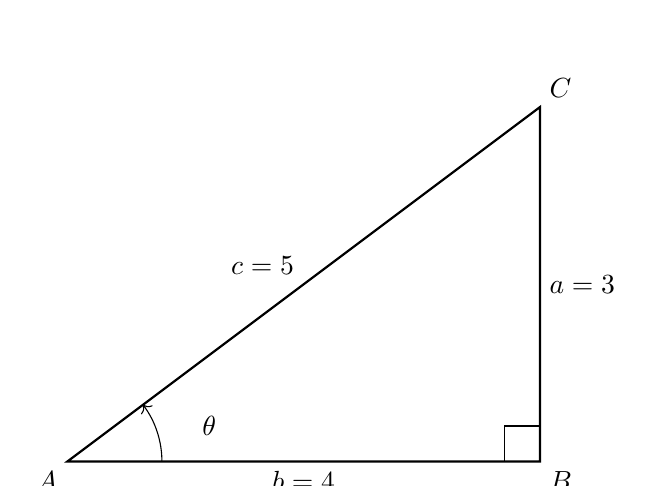
\begin{tikzpicture}[scale=1.5]
  % Triángulo rectángulo
  \coordinate (A) at (0,0);
  \coordinate (B) at (4,0);
  \coordinate (C) at (4,3);
  
  % Dibujar el triángulo
  \draw[thick] (A) -- (B) -- (C) -- cycle;
  
  % Ángulo recto
  \draw (3.7,0) -- (3.7,0.3) -- (4,0.3);
  
  % Etiquetas de vértices
  \node[below left] at (A) {$A$};
  \node[below right] at (B) {$B$};
  \node[above right] at (C) {$C$};
  
  % Etiquetas de lados
  \node[below] at (2,0) {$b = 4$};
  \node[right] at (4,1.5) {$a = 3$};
  \node[above left] at (2,1.5) {$c = 5$};
  
  % Ángulo
  \draw[->] (0.8,0) arc (0:36.87:0.8);
  \node at (1.2,0.3) {$\theta$};
\end{tikzpicture}
\end{center}

En este triángulo: \(c^2 = a^2 + b^2 = 9 + 16 = 25\), por lo tanto \(c = 5\).

\subsection{Ilustración: Círculo unitario con ángulos}

\begin{center}
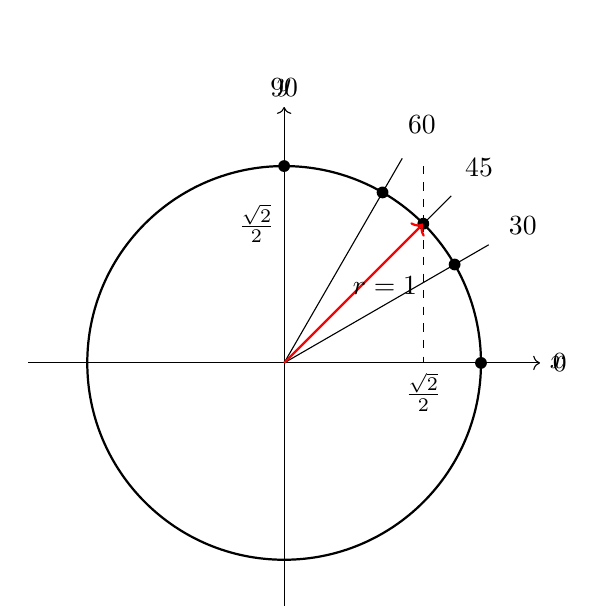
\begin{tikzpicture}[scale=2.5]
  % Círculo unitario
  \draw[thick] (0,0) circle (1);
  
  % Ejes
  \draw[->] (-1.3,0) -- (1.3,0) node[right] {$x$};
  \draw[->] (0,-1.3) -- (0,1.3) node[above] {$y$};
  
  % Ángulos importantes
  \foreach \angle/\label in {0/$0°$, 30/$30°$, 45/$45°$, 60/$60°$, 90/$90°$} {
    \draw (0,0) -- (\angle:1.2);
    \fill (\angle:1) circle (0.03);
    \node at (\angle:1.4) {\label};
  }
  
  % Punto en 45 grados
  \draw[thick, red, ->] (0,0) -- (45:1);
  \draw[dashed] (45:1) -- (45:1 |- 0,0);
  \draw[dashed] (45:1) -- (0,1 -| 45:1);
  
  % Coordenadas
  \node[below] at (0.707,0) {$\frac{\sqrt{2}}{2}$};
  \node[left] at (0,0.707) {$\frac{\sqrt{2}}{2}$};
  
  % Etiqueta del radio
  \node[above right] at (0.3,0.3) {$r=1$};
\end{tikzpicture}
\end{center}

El círculo unitario muestra que \(\sin(45°) = \cos(45°) = \frac{\sqrt{2}}{2}\).

\subsection{Ilustración: Parábola}

\begin{center}
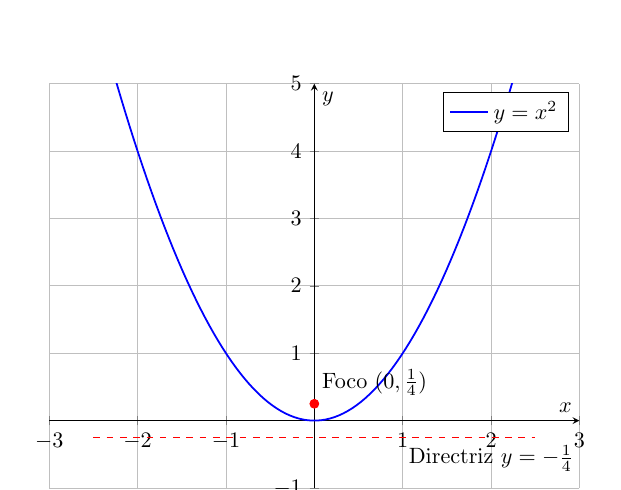
\begin{tikzpicture}[scale=0.8]
  \begin{axis}[
    axis lines = center,
    xlabel = {$x$},
    ylabel = {$y$},
    xmin=-3, xmax=3,
    ymin=-1, ymax=5,
    grid=major,
    width=10cm,
    height=8cm
  ]
  
  \addplot[
    domain=-2.5:2.5,
    samples=100,
    color=blue,
    thick
  ]{x^2};
  
  \addlegendentry{$y = x^2$}
  
  % Punto focal
  \addplot[mark=*, color=red] coordinates {(0,0.25)};
  \node[above right] at (axis cs:0,0.25) {Foco $(0, \frac{1}{4})$};
  
  % Directriz
  \addplot[color=red, dashed, domain=-2.5:2.5] {-0.25};
  \node[below] at (axis cs:2,-0.25) {Directriz $y = -\frac{1}{4}$};
  
  \end{axis}
\end{tikzpicture}
\end{center}

Parábola \(y = x^2\) con ecuación \(x^2 = 4py\) donde \(p = \frac{1}{4}\).

\section{Sólidos Geométricos}

\subsection{Cubo (arista \(a\))}

\[
\boxed{
\begin{aligned}
\text{Volumen} &= a^3 \\[6pt]
\text{Área superficial} &= 6a^2 \\[6pt]
\text{Diagonal espacial} &= a\sqrt{3} \\[6pt]
\text{Diagonal de cara} &= a\sqrt{2}
\end{aligned}
}
\]

\subsection{Paralelepípedo rectangular (dimensiones \(a, b, c\))}

\[
\boxed{
\begin{aligned}
\text{Volumen} &= abc \\[6pt]
\text{Área superficial} &= 2(ab + ac + bc) \\[6pt]
\text{Diagonal espacial} &= \sqrt{a^2 + b^2 + c^2}
\end{aligned}
}
\]

\subsection{Esfera (radio \(r\))}

\[
\boxed{
\begin{aligned}
\text{Volumen} &= \frac{4}{3}\pi r^3 \\[6pt]
\text{Área superficial} &= 4\pi r^2
\end{aligned}
}
\]

\textbf{Ecuación de la esfera} (centro en \((h, k, l)\)):

\[
\boxed{
(x-h)^2 + (y-k)^2 + (z-l)^2 = r^2
}
\]

\subsection{Cilindro circular (radio \(r\), altura \(h\))}

\[
\boxed{
\begin{aligned}
\text{Volumen} &= \pi r^2 h \\[6pt]
\text{Área superficial} &= 2\pi r^2 + 2\pi rh = 2\pi r(r + h) \\[6pt]
\text{Área lateral} &= 2\pi rh
\end{aligned}
}
\]

\subsection{Cono circular (radio \(r\), altura \(h\), generatriz \(l\))}

\[
\boxed{
\begin{aligned}
\text{Volumen} &= \frac{1}{3}\pi r^2 h \\[6pt]
\text{Área superficial} &= \pi r^2 + \pi rl = \pi r(r + l) \\[6pt]
\text{Área lateral} &= \pi rl \\[6pt]
l &= \sqrt{r^2 + h^2}
\end{aligned}
}
\]

\subsection{Pirámide}

\textbf{Pirámide general} (área de base \(A_b\), altura \(h\)):

\[
\boxed{
\text{Volumen} = \frac{1}{3}A_b \cdot h
}
\]

\textbf{Pirámide cuadrada} (lado de base \(a\), altura \(h\)):

\[
\boxed{
\begin{aligned}
\text{Volumen} &= \frac{1}{3}a^2h \\[6pt]
\text{Apotema} &= \sqrt{h^2 + \left(\frac{a}{2}\right)^2}
\end{aligned}
}
\]

\subsection{Prisma}

\textbf{Prisma general} (área de base \(A_b\), altura \(h\)):

\[
\boxed{
\text{Volumen} = A_b \cdot h
}
\]

\textbf{Prisma triangular} (base con lados \(a, b, c\), altura \(h\)):

\[
\boxed{
\text{Volumen} = \frac{h}{4}\sqrt{(a+b+c)(-a+b+c)(a-b+c)(a+b-c)}
}
\]

\subsection{Tronco de cono (radios \(r_1, r_2\), altura \(h\))}

\[
\boxed{
\begin{aligned}
\text{Volumen} &= \frac{\pi h}{3}(r_1^2 + r_1r_2 + r_2^2) \\[6pt]
\text{Área lateral} &= \pi(r_1 + r_2)l
\end{aligned}
}
\]

donde \(l = \sqrt{h^2 + (r_1 - r_2)^2}\) es la generatriz.

\subsection{Toro (radio mayor \(R\), radio menor \(r\))}

\[
\boxed{
\begin{aligned}
\text{Volumen} &= 2\pi^2 Rr^2 \\[6pt]
\text{Área superficial} &= 4\pi^2 Rr
\end{aligned}
}
\]

\subsection{Casquete esférico (radio \(r\), altura \(h\))}

\[
\boxed{
\begin{aligned}
\text{Volumen} &= \frac{\pi h^2}{3}(3r - h) \\[6pt]
\text{Área superficial} &= 2\pi rh
\end{aligned}
}
\]

\subsection{Elipsoide (semiejes \(a, b, c\))}

\[
\boxed{
\text{Volumen} = \frac{4}{3}\pi abc
}
\]

Si \(a = b\) (elipsoide de revolución):

\[
\boxed{
\text{Volumen} = \frac{4}{3}\pi a^2c
}
\]

\section{Teoremas Importantes}

\subsection{Teorema de Tales}

Si tres o más rectas paralelas son cortadas por dos transversales, los segmentos determinados en una transversal son proporcionales a los correspondientes segmentos en la otra.

\[
\boxed{
\frac{AB}{BC} = \frac{A'B'}{B'C'}
}
\]

\subsection{Teorema de Pitágoras generalizado}

En un triángulo cualquiera:

\[
\boxed{
c^2 = a^2 + b^2 - 2ab\cos C
}
\]

Si \(C = 90°\), se reduce al teorema clásico: \(c^2 = a^2 + b^2\).

\subsection{Teorema de Stewart}

En un triángulo \(ABC\) con una ceviana \(AD\) que divide el lado \(BC\) en segmentos \(m\) y \(n\):

\[
\boxed{
b^2m + c^2n = a(d^2 + mn)
}
\]

donde \(d\) es la longitud de la ceviana.

\subsection{Teorema de la bisectriz}

La bisectriz interna de un ángulo de un triángulo divide al lado opuesto en segmentos proporcionales a los lados adyacentes:

\[
\boxed{
\frac{BD}{DC} = \frac{AB}{AC}
}
\]

\subsection{Teorema de Menelao}

Para un triángulo \(ABC\) y una recta que corta los lados (o sus extensiones) en puntos \(D, E, F\):

\[
\boxed{
\frac{AF}{FB} \cdot \frac{BD}{DC} \cdot \frac{CE}{EA} = 1
}
\]

\subsection{Teorema de Ceva}

Tres cevianas \(AD, BE, CF\) de un triángulo \(ABC\) son concurrentes si y solo si:

\[
\boxed{
\frac{AF}{FB} \cdot \frac{BD}{DC} \cdot \frac{CE}{EA} = 1
}
\]

\subsection{Teorema de Euler (para triángulos)}

La distancia \(d\) entre el circuncentro \(O\) y el incentro \(I\) es:

\[
\boxed{
d^2 = R(R - 2r)
}
\]

donde \(R\) es el radio circunscrito y \(r\) el radio inscrito.

\subsection{Teorema del ángulo inscrito}

Un ángulo inscrito en un círculo mide la mitad del ángulo central que subtiende el mismo arco:

\[
\boxed{
\angle ACB = \frac{1}{2}\angle AOB
}
\]

\subsection{Teorema de Ptolomeo}

En un cuadrilátero cíclico con lados \(a, b, c, d\) y diagonales \(p, q\):

\[
\boxed{
pq = ac + bd
}
\]

\section{Funciones Trigonométricas Inversas}

\subsection{Dominios y rangos}

\[
\boxed{
\begin{aligned}
\arcsin(x) &: [-1, 1] \to \left[-\frac{\pi}{2}, \frac{\pi}{2}\right] \\[6pt]
\arccos(x) &: [-1, 1] \to [0, \pi] \\[6pt]
\arctan(x) &: \mathbb{R} \to \left(-\frac{\pi}{2}, \frac{\pi}{2}\right)
\end{aligned}
}
\]

\subsection{Identidades de funciones inversas}

\[
\boxed{
\begin{aligned}
\sin(\arcsin x) &= x \\[6pt]
\cos(\arccos x) &= x \\[6pt]
\tan(\arctan x) &= x \\[6pt]
\arcsin(\sin x) &= x \quad \text{si } x \in \left[-\frac{\pi}{2}, \frac{\pi}{2}\right] \\[6pt]
\arccos(\cos x) &= x \quad \text{si } x \in [0, \pi] \\[6pt]
\arctan(\tan x) &= x \quad \text{si } x \in \left(-\frac{\pi}{2}, \frac{\pi}{2}\right)
\end{aligned}
}
\]

\subsection{Relaciones entre funciones inversas}

\[
\boxed{
\begin{aligned}
\arcsin x + \arccos x &= \frac{\pi}{2} \\[6pt]
\arctan x + \arctan\frac{1}{x} &= \frac{\pi}{2} \quad (x > 0) \\[6pt]
\arctan x + \arctan y &= \arctan\frac{x+y}{1-xy} \quad (xy < 1)
\end{aligned}
}
\]

\subsection{Derivadas de funciones trigonométricas}

\[
\boxed{
\begin{aligned}
\frac{d}{dx}[\sin x] &= \cos x \\[6pt]
\frac{d}{dx}[\cos x] &= -\sin x \\[6pt]
\frac{d}{dx}[\tan x] &= \sec^2 x \\[6pt]
\frac{d}{dx}[\cot x] &= -\csc^2 x \\[6pt]
\frac{d}{dx}[\sec x] &= \sec x \tan x \\[6pt]
\frac{d}{dx}[\csc x] &= -\csc x \cot x
\end{aligned}
}
\]

\subsection{Derivadas de funciones trigonométricas inversas}

\[
\boxed{
\begin{aligned}
\frac{d}{dx}[\arcsin x] &= \frac{1}{\sqrt{1-x^2}} \\[6pt]
\frac{d}{dx}[\arccos x] &= -\frac{1}{\sqrt{1-x^2}} \\[6pt]
\frac{d}{dx}[\arctan x] &= \frac{1}{1+x^2}
\end{aligned}
}
\]

\section{Funciones Hiperbólicas}

\subsection{Definiciones}

\[
\boxed{
\begin{aligned}
\sinh x &= \frac{e^x - e^{-x}}{2} \\[6pt]
\cosh x &= \frac{e^x + e^{-x}}{2} \\[6pt]
\tanh x &= \frac{\sinh x}{\cosh x} = \frac{e^x - e^{-x}}{e^x + e^{-x}} \\[6pt]
\coth x &= \frac{\cosh x}{\sinh x} = \frac{e^x + e^{-x}}{e^x - e^{-x}} \\[6pt]
\text{sech}\, x &= \frac{1}{\cosh x} = \frac{2}{e^x + e^{-x}} \\[6pt]
\text{csch}\, x &= \frac{1}{\sinh x} = \frac{2}{e^x - e^{-x}}
\end{aligned}
}
\]

\subsection{Identidades hiperbólicas}

\[
\boxed{
\begin{aligned}
\cosh^2 x - \sinh^2 x &= 1 \\[6pt]
1 - \tanh^2 x &= \text{sech}^2 x \\[6pt]
\coth^2 x - 1 &= \text{csch}^2 x \\[6pt]
\sinh(2x) &= 2\sinh x \cosh x \\[6pt]
\cosh(2x) &= \cosh^2 x + \sinh^2 x = 2\cosh^2 x - 1 = 1 + 2\sinh^2 x
\end{aligned}
}
\]

\subsection{Suma y resta de funciones hiperbólicas}

\[
\boxed{
\begin{aligned}
\sinh(x \pm y) &= \sinh x \cosh y \pm \cosh x \sinh y \\[6pt]
\cosh(x \pm y) &= \cosh x \cosh y \pm \sinh x \sinh y \\[6pt]
\tanh(x \pm y) &= \frac{\tanh x \pm \tanh y}{1 \pm \tanh x \tanh y}
\end{aligned}
}
\]

\subsection{Derivadas de funciones hiperbólicas}

\[
\boxed{
\begin{aligned}
\frac{d}{dx}[\sinh x] &= \cosh x \\[6pt]
\frac{d}{dx}[\cosh x] &= \sinh x \\[6pt]
\frac{d}{dx}[\tanh x] &= \text{sech}^2 x \\[6pt]
\frac{d}{dx}[\coth x] &= -\text{csch}^2 x \\[6pt]
\frac{d}{dx}[\text{sech}\, x] &= -\text{sech}\, x \tanh x \\[6pt]
\frac{d}{dx}[\text{csch}\, x] &= -\text{csch}\, x \coth x
\end{aligned}
}
\]

\subsection{Funciones hiperbólicas inversas}

\[
\boxed{
\begin{aligned}
\text{arcsinh}\, x &= \ln(x + \sqrt{x^2 + 1}) \\[6pt]
\text{arccosh}\, x &= \ln(x + \sqrt{x^2 - 1}) \quad (x \geq 1) \\[6pt]
\text{arctanh}\, x &= \frac{1}{2}\ln\frac{1+x}{1-x} \quad (|x| < 1)
\end{aligned}
}
\]

\section{Coordenadas Polares}

\subsection{Conversión entre cartesianas y polares}

\textbf{De polares $(r, \theta)$ a cartesianas $(x, y)$}:

\[
\boxed{
\begin{aligned}
x &= r\cos\theta \\
y &= r\sin\theta
\end{aligned}
}
\]

\textbf{De cartesianas $(x, y)$ a polares $(r, \theta)$}:

\[
\boxed{
\begin{aligned}
r &= \sqrt{x^2 + y^2} \\
\theta &= \arctan\frac{y}{x}
\end{aligned}
}
\]

\subsection{Área en coordenadas polares}

Para una curva \(r = f(\theta)\) entre \(\theta = \alpha\) y \(\theta = \beta\):

\[
\boxed{
A = \frac{1}{2}\int_{\alpha}^{\beta} r^2 \, d\theta = \frac{1}{2}\int_{\alpha}^{\beta} [f(\theta)]^2 \, d\theta
}
\]

\subsection{Longitud de arco en polares}

\[
\boxed{
L = \int_{\alpha}^{\beta} \sqrt{r^2 + \left(\frac{dr}{d\theta}\right)^2} \, d\theta
}
\]

\subsection{Curvas polares comunes}

\textbf{Círculo}: \(r = a\)

\textbf{Espiral de Arquímedes}: \(r = a\theta\)

\textbf{Rosa de pétalos}: \(r = a\sin(n\theta)\) o \(r = a\cos(n\theta)\)

\textbf{Cardioide}: \(r = a(1 + \cos\theta)\)

\textbf{Lemniscata}: \(r^2 = a^2\cos(2\theta)\)

\textbf{Limaçon}: \(r = a + b\cos\theta\)

\subsection{Ilustración: Rosa polar de 4 pétalos}

\begin{center}
\begin{tikzpicture}[scale=1.5]
  \begin{axis}[
    axis equal,
    axis lines = none,
    xmin=-1.2, xmax=1.2,
    ymin=-1.2, ymax=1.2,
  ]
  
  \addplot[
    data cs=polar,
    domain=0:360,
    samples=200,
    color=purple,
    thick
  ] (x, {cos(2*x)});
  
  \end{axis}
  \node at (0,-2.5) {Rosa polar: $r = \cos(2\theta)$};
\end{tikzpicture}
\end{center}

\subsection{Ilustración: Cardioide}

\begin{center}
\begin{tikzpicture}[scale=1.2]
  \begin{axis}[
    axis equal,
    axis lines = none,
    xmin=-0.5, xmax=2.5,
    ymin=-1.5, ymax=1.5,
  ]
  
  \addplot[
    data cs=polar,
    domain=0:360,
    samples=200,
    color=red,
    thick
  ] (x, {1 + cos(x)});
  
  \end{axis}
  \node at (1.5,-2) {Cardioide: $r = 1 + \cos\theta$};
\end{tikzpicture}
\end{center}

\section{Coordenadas Esféricas y Cilíndricas}

\subsection{Coordenadas cilíndricas $(r, \theta, z)$}

\textbf{A cartesianas}:

\[
\boxed{
\begin{aligned}
x &= r\cos\theta \\
y &= r\sin\theta \\
z &= z
\end{aligned}
}
\]

\textbf{De cartesianas}:

\[
\boxed{
\begin{aligned}
r &= \sqrt{x^2 + y^2} \\
\theta &= \arctan\frac{y}{x} \\
z &= z
\end{aligned}
}
\]

\subsection{Coordenadas esféricas $(\rho, \theta, \phi)$}

\textbf{A cartesianas}:

\[
\boxed{
\begin{aligned}
x &= \rho\sin\phi\cos\theta \\
y &= \rho\sin\phi\sin\theta \\
z &= \rho\cos\phi
\end{aligned}
}
\]

\textbf{De cartesianas}:

\[
\boxed{
\begin{aligned}
\rho &= \sqrt{x^2 + y^2 + z^2} \\
\theta &= \arctan\frac{y}{x} \\
\phi &= \arccos\frac{z}{\sqrt{x^2 + y^2 + z^2}}
\end{aligned}
}
\]

\subsection{Elemento de volumen}

\textbf{Cilíndricas}: \(dV = r \, dr \, d\theta \, dz\)

\textbf{Esféricas}: \(dV = \rho^2 \sin\phi \, d\rho \, d\theta \, d\phi\)

\section{Series de Fourier}

\subsection{Serie de Fourier trigonométrica}

Para una función periódica \(f(x)\) con período \(2L\):

\[
\boxed{
f(x) = \frac{a_0}{2} + \sum_{n=1}^{\infty}\left[a_n\cos\frac{n\pi x}{L} + b_n\sin\frac{n\pi x}{L}\right]
}
\]

donde:

\[
\boxed{
\begin{aligned}
a_0 &= \frac{1}{L}\int_{-L}^{L} f(x) \, dx \\[6pt]
a_n &= \frac{1}{L}\int_{-L}^{L} f(x)\cos\frac{n\pi x}{L} \, dx \\[6pt]
b_n &= \frac{1}{L}\int_{-L}^{L} f(x)\sin\frac{n\pi x}{L} \, dx
\end{aligned}
}
\]

\subsection{Serie de Fourier compleja}

\[
\boxed{
f(x) = \sum_{n=-\infty}^{\infty} c_n e^{in\pi x/L}
}
\]

donde:

\[
\boxed{
c_n = \frac{1}{2L}\int_{-L}^{L} f(x)e^{-in\pi x/L} \, dx
}
\]

\section{Desigualdades Geométricas}

\subsection{Desigualdad entre medias}

Para números positivos \(a_1, a_2, \ldots, a_n\):

\[
\boxed{
\text{MH} \leq \text{MG} \leq \text{MA} \leq \text{MC}
}
\]

donde:

\begin{itemize}
  \item Media armónica: \(\text{MH} = \frac{n}{\frac{1}{a_1} + \frac{1}{a_2} + \cdots + \frac{1}{a_n}}\)
  \item Media geométrica: \(\text{MG} = \sqrt[n]{a_1 a_2 \cdots a_n}\)
  \item Media aritmética: \(\text{MA} = \frac{a_1 + a_2 + \cdots + a_n}{n}\)
  \item Media cuadrática: \(\text{MC} = \sqrt{\frac{a_1^2 + a_2^2 + \cdots + a_n^2}{n}}\)
\end{itemize}

\subsection{Desigualdad de Cauchy-Schwarz}

Para vectores \(\vec{u}\) y \(\vec{v}\):

\[
\boxed{
|\vec{u} \cdot \vec{v}| \leq |\vec{u}||\vec{v}|
}
\]

En forma de suma:

\[
\boxed{
\left(\sum_{i=1}^{n} a_i b_i\right)^2 \leq \left(\sum_{i=1}^{n} a_i^2\right)\left(\sum_{i=1}^{n} b_i^2\right)
}
\]

\subsection{Desigualdad del triángulo}

Para vectores:

\[
\boxed{
|\vec{u} + \vec{v}| \leq |\vec{u}| + |\vec{v}|
}
\]

Para números complejos \(z_1, z_2\):

\[
\boxed{
|z_1 + z_2| \leq |z_1| + |z_2|
}
\]

\subsection{Desigualdad isoperimétrica}

Para una figura plana con perímetro \(P\) y área \(A\):

\[
\boxed{
P^2 \geq 4\pi A
}
\]

con igualdad solo para el círculo.

\subsection{Desigualdad de Weitzenböck}

Para un triángulo con lados \(a, b, c\) y área \(S\):

\[
\boxed{
a^2 + b^2 + c^2 \geq 4\sqrt{3}S
}
\]

con igualdad solo para triángulos equiláteros.

\section{Números Complejos en Geometría}

\subsection{Forma rectangular}

\[
\boxed{
z = x + iy = \text{Re}(z) + i\text{Im}(z)
}
\]

\subsection{Forma polar}

\[
\boxed{
z = r(\cos\theta + i\sin\theta) = r\,\text{cis}\,\theta = re^{i\theta}
}
\]

donde:

\[
\boxed{
r = |z| = \sqrt{x^2 + y^2} \quad , \quad \theta = \arg(z) = \arctan\frac{y}{x}
}
\]

\subsection{Fórmula de Euler}

\[
\boxed{
e^{i\theta} = \cos\theta + i\sin\theta
}
\]

\subsection{Teorema de De Moivre}

\[
\boxed{
(\cos\theta + i\sin\theta)^n = \cos(n\theta) + i\sin(n\theta)
}
\]

o equivalentemente:

\[
\boxed{
(e^{i\theta})^n = e^{in\theta}
}
\]

\subsection{Raíces n-ésimas de la unidad}

Las \(n\) raíces de \(z^n = 1\) son:

\[
\boxed{
z_k = e^{2\pi ik/n} = \cos\frac{2\pi k}{n} + i\sin\frac{2\pi k}{n} \quad , \quad k = 0, 1, 2, \ldots, n-1
}
\]

\subsection{Raíces n-ésimas de un número complejo}

Las \(n\) raíces de \(z^n = w\) donde \(w = re^{i\theta}\) son:

\[
\boxed{
z_k = \sqrt[n]{r} \cdot e^{i(\theta + 2\pi k)/n} \quad , \quad k = 0, 1, 2, \ldots, n-1
}
\]

\section{Geometría Fractal}

\subsection{Dimensión fractal (dimensión de Hausdorff)}

\[
\boxed{
D = \frac{\log N}{\log(1/r)}
}
\]

donde \(N\) es el número de copias autosimilares y \(r\) es el factor de escala.

\subsection{Ejemplos de dimensiones fractales}

\begin{itemize}
  \item Línea recta: \(D = 1\)
  \item Conjunto de Cantor: \(D = \frac{\log 2}{\log 3} \approx 0.631\)
  \item Curva de Koch: \(D = \frac{\log 4}{\log 3} \approx 1.262\)
  \item Triángulo de Sierpinski: \(D = \frac{\log 3}{\log 2} \approx 1.585\)
  \item Esponja de Menger: \(D = \frac{\log 20}{\log 3} \approx 2.727\)
\end{itemize}

\section{Transformaciones Lineales y Matrices}

\subsection{Matriz de rotación en 2D}

Rotación por ángulo \(\theta\):

\[
\boxed{
R(\theta) = \begin{pmatrix} \cos\theta & -\sin\theta \\ \sin\theta & \cos\theta \end{pmatrix}
}
\]

\subsection{Matriz de rotación en 3D}

\textbf{Alrededor del eje \(x\)}:

\[
\boxed{
R_x(\theta) = \begin{pmatrix}
1 & 0 & 0 \\
0 & \cos\theta & -\sin\theta \\
0 & \sin\theta & \cos\theta
\end{pmatrix}
}
\]

\textbf{Alrededor del eje \(y\)}:

\[
\boxed{
R_y(\theta) = \begin{pmatrix}
\cos\theta & 0 & \sin\theta \\
0 & 1 & 0 \\
-\sin\theta & 0 & \cos\theta
\end{pmatrix}
}
\]

\textbf{Alrededor del eje \(z\)}:

\[
\boxed{
R_z(\theta) = \begin{pmatrix}
\cos\theta & -\sin\theta & 0 \\
\sin\theta & \cos\theta & 0 \\
0 & 0 & 1
\end{pmatrix}
}
\]

\subsection{Matriz de reflexión}

\textbf{Respecto al eje \(x\)}:

\[
\boxed{
M_x = \begin{pmatrix} 1 & 0 \\ 0 & -1 \end{pmatrix}
}
\]

\textbf{Respecto al eje \(y\)}:

\[
\boxed{
M_y = \begin{pmatrix} -1 & 0 \\ 0 & 1 \end{pmatrix}
}
\]

\textbf{Respecto al origen}:

\[
\boxed{
M_O = \begin{pmatrix} -1 & 0 \\ 0 & -1 \end{pmatrix}
}
\]

\subsection{Matriz de escalamiento}

\[
\boxed{
S(s_x, s_y) = \begin{pmatrix} s_x & 0 \\ 0 & s_y \end{pmatrix}
}
\]

\subsection{Matriz de cizallamiento (shear)}

\textbf{Horizontal}:

\[
\boxed{
H_x(k) = \begin{pmatrix} 1 & k \\ 0 & 1 \end{pmatrix}
}
\]

\textbf{Vertical}:

\[
\boxed{
H_y(k) = \begin{pmatrix} 1 & 0 \\ k & 1 \end{pmatrix}
}
\]

\section{Fórmulas Adicionales}

\subsection{Número de oro (phi)}

\[
\boxed{
\phi = \frac{1 + \sqrt{5}}{2} \approx 1.618033988749895
}
\]

Propiedades:

\[
\boxed{
\phi^2 = \phi + 1 \quad , \quad \frac{1}{\phi} = \phi - 1
}
\]

\subsection{Rectángulo áureo}

Un rectángulo con proporción \(\phi:1\).

\[
\boxed{
\frac{a+b}{a} = \frac{a}{b} = \phi
}
\]

\subsection{Espiral áurea}

Una espiral logarítmica que crece por un factor de \(\phi\) por cada cuarto de vuelta.

\subsection{Ángulo sólido}

Para una esfera completa:

\[
\boxed{
\Omega = 4\pi \text{ estereoradianes}
}
\]

Para un casquete esférico con ángulo \(\theta\):

\[
\boxed{
\Omega = 2\pi(1 - \cos\theta)
}
\]

\section{Aproximaciones Útiles}

Para ángulos pequeños \(x\) (en radianes):

\[
\boxed{
\begin{aligned}
\sin x &\approx x - \frac{x^3}{6} \approx x \\[6pt]
\cos x &\approx 1 - \frac{x^2}{2} \\[6pt]
\tan x &\approx x + \frac{x^3}{3} \approx x
\end{aligned}
}
\]

\section{Ilustración: Hexágono regular inscrito}

\begin{center}
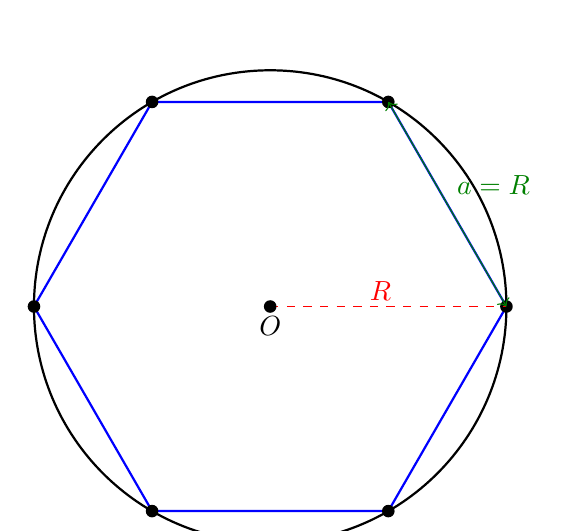
\begin{tikzpicture}[scale=2]
  % Círculo
  \draw[thick] (0,0) circle (1.5);
  
  % Hexágono
  \foreach \i in {0,1,...,5} {
    \coordinate (p\i) at ({60*\i}:1.5);
  }
  
  \draw[thick, blue] (p0) -- (p1) -- (p2) -- (p3) -- (p4) -- (p5) -- cycle;
  
  % Puntos
  \foreach \i in {0,1,...,5} {
    \fill ({60*\i}:1.5) circle (0.04);
  }
  
  % Radio
  \draw[red, dashed] (0,0) -- (p0);
  \node[red] at (0.7,0.1) {$R$};
  
  % Centro
  \fill (0,0) circle (0.04);
  \node[below] at (0,0) {$O$};
  
  % Lado
  \draw[green!50!black, <->] (p0) -- (p1);
  \node[green!50!black, above right] at ($(p0)!0.5!(p1)$) {$a = R$};
\end{tikzpicture}
\end{center}

En un hexágono regular inscrito en un círculo de radio \(R\), el lado del hexágono es igual al radio: \(a = R\).

\section{Geometría Computacional}

\subsection{Producto cruz en 2D (determinante)}

Para vectores \(\vec{u} = (u_x, u_y)\) y \(\vec{v} = (v_x, v_y)\):

\[
\boxed{
\vec{u} \times \vec{v} = u_x v_y - u_y v_x
}
\]

Resultado positivo: \(\vec{v}\) está a la izquierda de \(\vec{u}\)

Resultado negativo: \(\vec{v}\) está a la derecha de \(\vec{u}\)

Resultado cero: \(\vec{u}\) y \(\vec{v}\) son colineales

\subsection{Área de polígono por coordenadas}

Para un polígono con vértices \((x_1, y_1), (x_2, y_2), \ldots, (x_n, y_n)\):

\[
\boxed{
A = \frac{1}{2}\left|\sum_{i=1}^{n}(x_i y_{i+1} - x_{i+1} y_i)\right|
}
\]

donde \((x_{n+1}, y_{n+1}) = (x_1, y_1)\).

\subsection{Punto dentro de un polígono convexo}

Un punto \(P\) está dentro de un polígono convexo si tiene el mismo signo del producto cruz con todos los lados consecutivos.

\subsection{Punto dentro de un triángulo}

Un punto \(P(x, y)\) está dentro del triángulo \(ABC\) si:

\[
\boxed{
\alpha \geq 0, \, \beta \geq 0, \, \gamma \geq 0, \, \text{ y } \, \alpha + \beta + \gamma = 1
}
\]

donde \((\alpha, \beta, \gamma)\) son las coordenadas baricéntricas:

\[
P = \alpha A + \beta B + \gamma C
\]

\subsection{Convex Hull (Envolvente Convexa)}

Algoritmos comunes:
\begin{itemize}
  \item \textbf{Graham Scan}: \(O(n \log n)\)
  \item \textbf{Jarvis March (Gift Wrapping)}: \(O(nh)\) donde \(h\) es el número de puntos en el hull
  \item \textbf{Andrew's Algorithm}: \(O(n \log n)\)
\end{itemize}

\subsection{Intersección de segmentos}

Dos segmentos \(P_1P_2\) y \(P_3P_4\) se intersectan si:

\begin{itemize}
  \item Los puntos \(P_3\) y \(P_4\) están en lados opuestos de la línea \(P_1P_2\), Y
  \item Los puntos \(P_1\) y \(P_2\) están en lados opuestos de la línea \(P_3P_4\)
\end{itemize}

\subsection{Punto más cercano a un segmento}

Dado un punto \(P\) y un segmento \(AB\), el punto más cercano \(Q\) en \(AB\) a \(P\) es:

\[
\boxed{
Q = A + t(B - A)
}
\]

donde:

\[
\boxed{
t = \max\left(0, \min\left(1, \frac{(P-A) \cdot (B-A)}{|B-A|^2}\right)\right)
}
\]

\section{Distancias Especiales}

\subsection{Distancia de Manhattan}

\[
\boxed{
d_{\text{Manhattan}} = |x_2 - x_1| + |y_2 - y_1|
}
\]

\subsection{Distancia de Chebyshev}

\[
\boxed{
d_{\text{Chebyshev}} = \max(|x_2 - x_1|, |y_2 - y_1|)
}
\]

\subsection{Distancia de Minkowski}

\[
\boxed{
d_p = \left(\sum_{i=1}^{n}|x_i - y_i|^p\right)^{1/p}
}
\]

Casos especiales:
\begin{itemize}
  \item \(p = 1\): Distancia de Manhattan
  \item \(p = 2\): Distancia euclidiana
  \item \(p = \infty\): Distancia de Chebyshev
\end{itemize}

\subsection{Distancia de Hamming}

Número de posiciones en las que dos cadenas difieren.

\subsection{Distancia de Hausdorff}

Para dos conjuntos \(A\) y \(B\):

\[
\boxed{
d_H(A, B) = \max\left(\sup_{a \in A}\inf_{b \in B}d(a,b), \sup_{b \in B}\inf_{a \in A}d(a,b)\right)
}
\]

\section{Teoremas Avanzados}

\subsection{Teorema de Napoleon}

Si se construyen triángulos equiláteros sobre los lados de cualquier triángulo, los centros de estos triángulos equiláteros forman otro triángulo equilátero.

\subsection{Teorema de Morley}

Los tres puntos de intersección de los trisectores de ángulos adyacentes de cualquier triángulo forman un triángulo equilátero.

\subsection{Teorema del punto de Fermat}

Para un triángulo \(ABC\), el punto \(P\) que minimiza \(PA + PB + PC\) es el punto de Fermat, donde:
\begin{itemize}
  \item Si todos los ángulos son \(< 120°\), entonces \(\angle APB = \angle BPC = \angle CPA = 120°\)
  \item Si un ángulo es \(\geq 120°\), el punto de Fermat es ese vértice
\end{itemize}

\subsection{Teorema de Feuerbach (Círculo de los nueve puntos)}

El círculo que pasa por:
\begin{itemize}
  \item Los puntos medios de los tres lados
  \item Los pies de las tres alturas
  \item Los puntos medios entre vértices y ortocentro
\end{itemize}

Este círculo tiene radio \(R/2\) donde \(R\) es el radio circunscrito.

\subsection{Teorema de Carnot}

En un triángulo \(ABC\) con circuncentro \(O\) y alturas \(h_a, h_b, h_c\):

\[
\boxed{
OA^2 + OB^2 + OC^2 = R^2(1 + \cos A + \cos B + \cos C)
}
\]

\subsection{Teorema de Menelao generalizado (3D)}

Para un tetraedro y un plano que lo corta, el producto de las razones de división es \(-1\).

\subsection{Identidad de Brahmagupta}

\[
\boxed{
(a^2 + b^2)(c^2 + d^2) = (ac - bd)^2 + (ad + bc)^2 = (ac + bd)^2 + (ad - bc)^2
}
\]

\subsection{Teorema japonés}

En cualquier cuadrilátero cíclico dividido en triángulos por sus diagonales, la suma de los radios de los círculos inscritos en los triángulos opuestos es constante.

\section{Fórmulas de Área Avanzadas}

\subsection{Área de un cuadrilátero con diagonales}

Para un cuadrilátero con diagonales \(p\) y \(q\) que se intersectan con ángulo \(\theta\):

\[
\boxed{
A = \frac{1}{2}pq\sin\theta
}
\]

\subsection{Fórmula de Coolidge para cuadriláteros}

\[
\boxed{
16A^2 = 4p^2q^2 - (b^2 + d^2 - a^2 - c^2)^2
}
\]

donde \(a, b, c, d\) son los lados y \(p, q\) las diagonales.

\subsection{Área de un polígono regular}

Para un polígono regular de \(n\) lados con lado \(a\):

\[
\boxed{
A = \frac{na^2}{4\tan(\pi/n)}
}
\]

\subsection{Área de un sector elíptico}

No tiene fórmula cerrada simple, pero se puede aproximar usando integrales elípticas.

\section{Centros Notables del Triángulo}

\subsection{Ortocentro (H)}

Intersección de las tres alturas.

\textbf{Coordenadas}:
\[
H = \left(\frac{\tan A \cdot x_A + \tan B \cdot x_B + \tan C \cdot x_C}{\tan A + \tan B + \tan C}, \ldots\right)
\]

\subsection{Circuncentro (O)}

Intersección de las mediatrices.

\textbf{Coordenadas}:
\[
O = \left(\frac{x_A\sin 2A + x_B\sin 2B + x_C\sin 2C}{\sin 2A + \sin 2B + \sin 2C}, \ldots\right)
\]

\subsection{Incentro (I)}

Intersección de las bisectrices internas.

\textbf{Coordenadas baricéntricas}:
\[
\boxed{
I = \frac{aA + bB + cC}{a + b + c}
}
\]

\subsection{Baricentro (G)}

Intersección de las medianas. Es el centro de masa.

\textbf{Coordenadas}:
\[
\boxed{
G = \left(\frac{x_A + x_B + x_C}{3}, \frac{y_A + y_B + y_C}{3}\right)
}
\]

\subsection{Recta de Euler}

El ortocentro \(H\), circuncentro \(O\) y baricentro \(G\) son colineales, con:

\[
\boxed{
\overrightarrow{OG} = \frac{1}{3}\overrightarrow{OH}
}
\]

Es decir, \(G\) divide el segmento \(OH\) en razón \(1:2\).

\section{Secciones Cónicas - Propiedades Avanzadas}

\subsection{Ecuación general de una cónica}

\[
\boxed{
Ax^2 + Bxy + Cy^2 + Dx + Ey + F = 0
}
\]

\textbf{Discriminante}:
\[
\Delta = B^2 - 4AC
\]

\begin{itemize}
  \item \(\Delta < 0\): Elipse (o círculo si \(A = C\) y \(B = 0\))
  \item \(\Delta = 0\): Parábola
  \item \(\Delta > 0\): Hipérbola
\end{itemize}

\subsection{Propiedades focales de la parábola}

Todo rayo paralelo al eje de la parábola se refleja hacia el foco.

\subsection{Propiedades focales de la elipse}

La suma de distancias desde cualquier punto de la elipse a los dos focos es constante e igual a \(2a\).

\subsection{Propiedades focales de la hipérbola}

La diferencia absoluta de distancias desde cualquier punto de la hipérbola a los dos focos es constante e igual a \(2a\).

\subsection{Tangente a una cónica}

Para la elipse \(\frac{x^2}{a^2} + \frac{y^2}{b^2} = 1\) en el punto \((x_0, y_0)\):

\[
\boxed{
\frac{xx_0}{a^2} + \frac{yy_0}{b^2} = 1
}
\]

Para la hipérbola \(\frac{x^2}{a^2} - \frac{y^2}{b^2} = 1\) en el punto \((x_0, y_0)\):

\[
\boxed{
\frac{xx_0}{a^2} - \frac{yy_0}{b^2} = 1
}
\]

Para la parábola \(y^2 = 4px\) en el punto \((x_0, y_0)\):

\[
\boxed{
yy_0 = 2p(x + x_0)
}
\]

\section{Curvas Paramétricas}

\subsection{Cicloide}

Curva trazada por un punto en un círculo que rueda:

\[
\boxed{
\begin{aligned}
x &= r(\theta - \sin\theta) \\
y &= r(1 - \cos\theta)
\end{aligned}
}
\]

\subsection{Epicicloide}

\[
\boxed{
\begin{aligned}
x &= (R + r)\cos\theta - r\cos\left(\frac{R + r}{r}\theta\right) \\
y &= (R + r)\sin\theta - r\sin\left(\frac{R + r}{r}\theta\right)
\end{aligned}
}
\]

\subsection{Hipocicloide}

\[
\boxed{
\begin{aligned}
x &= (R - r)\cos\theta + r\cos\left(\frac{R - r}{r}\theta\right) \\
y &= (R - r)\sin\theta - r\sin\left(\frac{R - r}{r}\theta\right)
\end{aligned}
}
\]

\subsection{Astroide (Hipocicloide con \(R = 4r\))}

\[
\boxed{
x^{2/3} + y^{2/3} = a^{2/3}
}
\]

Forma paramétrica:
\[
\boxed{
x = a\cos^3 t \quad , \quad y = a\sin^3 t
}
\]

\subsection{Lemniscata de Bernoulli}

\[
\boxed{
(x^2 + y^2)^2 = a^2(x^2 - y^2)
}
\]

En polares:
\[
\boxed{
r^2 = a^2\cos(2\theta)
}
\]

\section{Curvatura}

\subsection{Curvatura de una curva plana}

Para una curva \(y = f(x)\):

\[
\boxed{
\kappa = \frac{|f''(x)|}{(1 + [f'(x)]^2)^{3/2}}
}
\]

Para una curva paramétrica \((x(t), y(t))\):

\[
\boxed{
\kappa = \frac{|x'y'' - y'x''|}{(x'^2 + y'^2)^{3/2}}
}
\]

\subsection{Radio de curvatura}

\[
\boxed{
\rho = \frac{1}{\kappa}
}
\]

\subsection{Curvatura del círculo}

Para un círculo de radio \(r\):

\[
\boxed{
\kappa = \frac{1}{r}
}
\]

\section{Superficies Cuádricas}

\subsection{Elipsoide}

\[
\boxed{
\frac{x^2}{a^2} + \frac{y^2}{b^2} + \frac{z^2}{c^2} = 1
}
\]

\subsection{Hiperboloide de una hoja}

\[
\boxed{
\frac{x^2}{a^2} + \frac{y^2}{b^2} - \frac{z^2}{c^2} = 1
}
\]

\subsection{Hiperboloide de dos hojas}

\[
\boxed{
\frac{x^2}{a^2} + \frac{y^2}{b^2} - \frac{z^2}{c^2} = -1
}
\]

\subsection{Paraboloide elíptico}

\[
\boxed{
\frac{x^2}{a^2} + \frac{y^2}{b^2} = z
}
\]

\subsection{Paraboloide hiperbólico (silla de montar)}

\[
\boxed{
\frac{x^2}{a^2} - \frac{y^2}{b^2} = z
}
\]

\subsection{Cono elíptico}

\[
\boxed{
\frac{x^2}{a^2} + \frac{y^2}{b^2} = \frac{z^2}{c^2}
}
\]

\section{Ilustración: Funciones trigonométricas}

\begin{center}
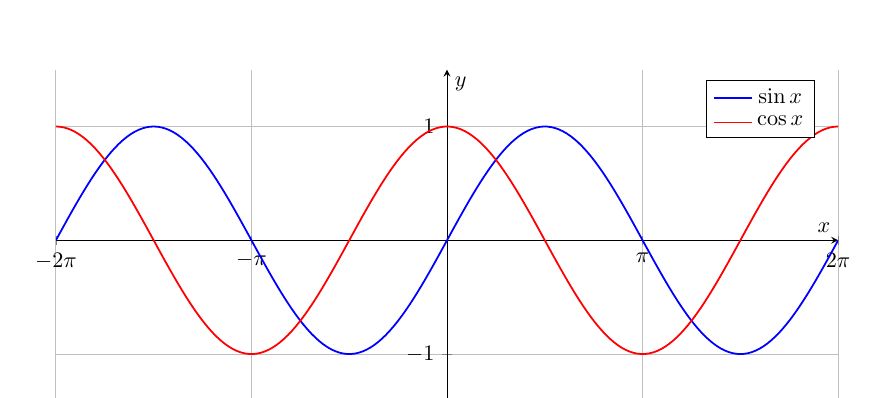
\begin{tikzpicture}[scale=0.8]
  \begin{axis}[
    axis lines = middle,
    xlabel = {$x$},
    ylabel = {$y$},
    xmin=-2*pi, xmax=2*pi,
    ymin=-1.5, ymax=1.5,
    xtick={-6.28318, -3.14159, 0, 3.14159, 6.28318},
    xticklabels={$-2\pi$, $-\pi$, $0$, $\pi$, $2\pi$},
    grid=major,
    width=14cm,
    height=7cm,
    legend pos=north east
  ]
  
  \addplot[
    domain=-2*pi:2*pi,
    samples=200,
    color=blue,
    thick
  ]{sin(deg(x))};
  \addlegendentry{$\sin x$}
  
  \addplot[
    domain=-2*pi:2*pi,
    samples=200,
    color=red,
    thick
  ]{cos(deg(x))};
  \addlegendentry{$\cos x$}
  
  \end{axis}
\end{tikzpicture}
\end{center}

\section{Integrales Trigonométricas Útiles}

\[
\boxed{
\begin{aligned}
\int \sin x \, dx &= -\cos x + C \\[6pt]
\int \cos x \, dx &= \sin x + C \\[6pt]
\int \tan x \, dx &= -\ln|\cos x| + C = \ln|\sec x| + C \\[6pt]
\int \sec x \, dx &= \ln|\sec x + \tan x| + C \\[6pt]
\int \sec^2 x \, dx &= \tan x + C \\[6pt]
\int \csc^2 x \, dx &= -\cot x + C
\end{aligned}
}
\]

\section{Constantes Geométricas Importantes}

\[
\boxed{
\begin{aligned}
\pi &\approx 3.141592653589793 \\[6pt]
e &\approx 2.718281828459045 \\[6pt]
\phi &= \frac{1 + \sqrt{5}}{2} \approx 1.618033988749895 \\[6pt]
\sqrt{2} &\approx 1.414213562373095 \\[6pt]
\sqrt{3} &\approx 1.732050807568877 \\[6pt]
\sqrt{5} &\approx 2.236067977499790
\end{aligned}
}
\]

\section{Relaciones entre Trigonometría y Números Complejos}

\subsection{Identidades de Euler}

\[
\boxed{
\begin{aligned}
\cos x &= \frac{e^{ix} + e^{-ix}}{2} \\[6pt]
\sin x &= \frac{e^{ix} - e^{-ix}}{2i}
\end{aligned}
}
\]

\subsection{Fórmula más bella de las matemáticas}

\[
\boxed{
e^{i\pi} + 1 = 0
}
\]

Esta fórmula conecta cinco de las constantes matemáticas más importantes: \(e\), \(i\), \(\pi\), \(1\) y \(0\).

\section{Notas Finales}

Este documento contiene las fórmulas y teoremas más importantes de geometría y trigonometría. Es útil para:

\begin{itemize}
  \item Resolución rápida de problemas
  \item Competencias de matemáticas (Olimpiadas, ACM ICPC)
  \item Referencia académica
  \item Geometría computacional
  \item Gráficos por computadora
  \item Física e ingeniería
\end{itemize}

\vspace{1cm}

\begin{center}
\textit{``La geometría es el conocimiento de lo eternamente existente.''} \\
--- Platón
\end{center}

\end{document}
